\documentclass{article}
\usepackage[eandd]{neurips_2026}
\usepackage[T1]{fontenc}
\usepackage{url}
\usepackage{amsfonts}
\usepackage{nicefrac}
\usepackage{microtype}
\usepackage[utf8]{inputenc}
\usepackage{amsmath,amssymb}
\usepackage{booktabs}
\usepackage{hyperref}
\usepackage{graphicx}
\usepackage{listings}
\usepackage{xcolor}
\usepackage{enumitem}
\usepackage{caption}
\usepackage{subcaption}
\usepackage{tikz}
\usepackage{multirow}
\usetikzlibrary{arrows.meta,positioning,shapes.geometric}

\lstset{
  basicstyle=\ttfamily\small,
  backgroundcolor=\color{gray!10},
  frame=single,
  breaklines=true,
  columns=fullflexible,
  keywordstyle=\color{blue!70!black},
  commentstyle=\color{green!50!black},
  stringstyle=\color{red!60!black},
}

\title{\textbf{MLAuditBench}: An Interactive RL Environment for\\
Evaluating LLM Agents on ML Experiment Integrity Auditing}

\author{Anonymous Authors}

\begin{document}
\maketitle

\begin{abstract}
Machine learning research faces a well-documented reproducibility crisis.
Kapoor \& Narayanan (2023) identified data leakage in 294~papers across
17~scientific fields, and follow-up work expanded this to 648~papers across
30~fields.  Existing tools for detecting these violations rely on static
code analysis or post-hoc manual checklists.  We introduce
\textsc{MLAuditBench}, the first reinforcement learning environment that
frames ML experiment integrity auditing as an interactive agent task.
Agents must sequentially inspect experiment artifacts (preprocessing code,
split configurations, training logs, evaluation reports), identify
violations with evidence-grounded reasoning, and submit a verdict---all
within a step budget.  The environment implements 8 violation types drawn
from the reproducibility literature, spans 5 ML archetypes and 56 unique
experiments (v1.0; v1.1 extends to 62 across a text-classification
archetype) across 3 difficulty tiers, and uses a layered reward function
combining violation detection (80\%), audit efficiency (10\%), and verdict
accuracy (10\%).  Anti-gaming mechanisms include adversarially clean
experiments (50\%/35\%/20\% draw probability for easy/medium/hard) and red
herrings in harder tasks.  We evaluate three frontier OpenAI models
(GPT-4.1-mini, GPT-4.1, o4-mini) over 10 seeds each, an interactive
single-seed Claude Sonnet 4.6 expert audit, a preliminary open-weight
Qwen2.5-72B run, and a 10-seed \emph{ML-trained human baseline}
($0.82\pm0.13$ easy, $0.86\pm0.09$ medium, $0.57\pm0.34$ hard).
On primary seeds (45--46) GPT-4.1-mini and o4-mini match or exceed humans
on cross-artifact reasoning at the medium tier ($0.913$--$0.917$
vs.\ $0.86$ for humans) yet remain below the interactive Claude expert
ceiling ($0.954$) on compound hard-tier tasks.
Per-seed root-cause analysis identified nine inference-script failure modes
whose repair collapses GPT-4.1-mini easy/medium 10-seed variance from
$\sigma{=}0.39/0.34$ to $\sigma{=}0.00/0.003$; under the corrected
script, GPT-4.1-mini reaches $0.900/0.901/0.819$ across tiers, GPT-4.1
reaches $0.900/0.783/0.780$, and o4-mini ($0.539/0.588/0.469$) shows
no improvement, confirming model-level failures dominate for reasoning
models.  An evidence-matching threshold ablation across
$\{0.6,0.7,0.8,0.9,1.0\}$ confirms model rankings are stable under all
five thresholds.
The environment is deployed as an OpenEnv-compatible Docker container on
Hugging Face Spaces and is fully reproducible from the released seeds.
\end{abstract}

% ============================================================================
\section{Introduction}
\label{sec:intro}

The ML reproducibility crisis is not merely an academic inconvenience---it
produces unreliable results that propagate into deployed systems, medical
diagnoses, and policy decisions.  The seminal audit by Kapoor \&
Narayanan~\cite{kapoor2023leakage} established a taxonomy of 8 leakage
types and demonstrated their pervasive presence across scientific
disciplines, from health sciences to economics.  Their follow-up REFORMS
checklist~\cite{kapoor2024reforms} provides a 32-question consensus
framework, but its application remains manual and does not scale.

On the automated detection side, Yang et al.~\cite{yang2022data} pioneered
static data-flow analysis for Jupyter notebooks, finding approximately
30\% of 100,000+ public notebooks exhibit some form of leakage.
Drobnjakovi\'c et al.~\cite{drobnjakovic2024tase} advanced this with the
NBLyzer framework using abstract interpretation.  However, all existing
approaches are \emph{static}---they analyze code snapshots without
interactive reasoning.

We argue that ML experiment auditing is fundamentally an \emph{interactive
reasoning} task.  An auditor must: (1) decide which artifacts to examine
given limited time; (2) cross-reference information across artifacts (e.g.,
comparing feature lists against target columns); (3) distinguish genuine
violations from benign patterns that merely look suspicious; and (4)
synthesize evidence into a grounded verdict.  This sequential
decision-making structure maps naturally onto the reinforcement learning
framework.

\textsc{MLAuditBench} is, to our knowledge, the first RL environment
specifically designed for ML experiment integrity auditing.  It fills a
clear gap in the benchmark landscape: SWE-bench~\cite{jimenez2024swebench}
tests bug fixing, not methodology auditing; CORE-Bench tests computational
reproducibility, not violation detection; and SPOT evaluates error
detection in manuscripts, not in code artifacts.

\paragraph{Contributions.}
(i) We formalize ML experiment auditing as an interactive RL task with a
typed action/observation space, evidence-grounding requirements, and a
layered scoring function.
(ii) We implement 8 violation types spanning the full Kapoor \& Narayanan
taxonomy, instantiated across 5 ML archetypes in 56 unique experiments
(v1.0; extended to 62 in v1.1).
(iii) We provide anti-gaming mechanisms including adversarially clean
experiments and red herrings.
(iv) We evaluate three OpenAI model families (fast, balanced,
reasoning-optimised), an interactive Claude Sonnet 4.6 expert audit, a
preliminary open-weight Qwen2.5-72B baseline, and a 10-seed-per-tier
\emph{ML-trained human baseline} run under identical action schema, step
budget, and grader.  We provide bootstrap 95\% confidence intervals for
all numbers reported.
(v) We package the environment as an OpenEnv-compliant Docker container
deployable to Hugging Face Spaces and release a complete human-evaluation
kit (facilitator protocol, participant instructions, session-log
templates, and scoring scripts) so the community can reproduce or extend
the human comparison.

\paragraph{Paper organisation.}
Section~\ref{sec:related} surveys related work.
Section~\ref{sec:design} describes the environment design.
Section~\ref{sec:scoring} specifies the reward function and
Section~\ref{sec:eval} presents the evaluation protocol and results.
Sections~\ref{sec:human}--\ref{sec:fixes} analyse the human baseline,
variance, threshold sensitivity, and inference-script failure modes.
Section~\ref{sec:limitations} discusses limitations and future work.

% ============================================================================
\section{Related Work}
\label{sec:related}

\paragraph{ML Reproducibility Auditing.}
The foundational taxonomy by Kapoor \& Narayanan~\cite{kapoor2023leakage}
identified 8 leakage types across 17 fields.  Yang et al.~\cite{yang2022data}
implemented static detection via data-flow analysis (92.9\% accuracy on
notebooks).  Lones~\cite{lones2021avoid} provided a practical guideline
taxonomy.  Alali et al.~\cite{alali2025llmleakage} evaluated LLM-based
approaches using CodeBERT and GPT for adaptive static detection.

\paragraph{Agent Benchmarks.}
SWE-bench~\cite{jimenez2024swebench} (ICLR 2024) tests code bug-fixing
across 2,294 GitHub issues.  MLAgentBench~\cite{huang2024mlagentbench}
evaluates agents \emph{performing} ML experiments, not auditing them.
CORE-Bench~\cite{kapoor2024corebench} (TMLR 2025) tests computational
reproducibility by re-running existing code.  SPOT~\cite{spot2025}
evaluates error detection in scientific manuscripts (prose), not in code
artifacts.  None of these frames \emph{integrity auditing} as an
interactive RL task with evidence-grounded scoring \emph{and} reports a
matched human baseline.

\paragraph{Human Baselines for LLM Agents.}
Following the precedent established by SWE-bench (where humans are
implicitly the upper bound of \emph{written} fixes) and HumanEval, we
report a constraint-matched human baseline using identical action
schema, step budgets, and grader.  Our baseline is pitched explicitly as
a capability anchor and not as a claim of expert consensus.

\paragraph{RL Reward Design.}
Potential-based reward shaping~\cite{ng1999policy} provides the
theoretical foundation for our layered reward design.  Process reward
models~\cite{luo2025pitfalls} % TODO: verify AgentPRM citation key
and Shapley-value credit assignment inform our partial credit mechanisms.

\paragraph{Positioning.}
Table~\ref{tab:related} summarises how \textsc{MLAuditBench} differs from
the most similar benchmarks.

\begin{table}[h]
\centering
\caption{Comparison with related benchmarks. ``Human baseline'' = a
constraint-matched human reference run is reported in the original
release.}
\label{tab:related}
\small
\begin{tabular}{lccccc}
\toprule
\textbf{Benchmark} & \textbf{Interactive} & \textbf{Code-level} & \textbf{Violation Det.} & \textbf{Evidence-grounded} & \textbf{Human baseline} \\
\midrule
SWE-bench~\cite{jimenez2024swebench}      & \checkmark & \checkmark & \texttimes & \texttimes & \texttimes \\
CORE-Bench~\cite{kapoor2024corebench}     & \checkmark & \checkmark & \texttimes & \texttimes & \texttimes \\
MLAgentBench~\cite{huang2024mlagentbench} & \checkmark & \checkmark & \texttimes & \texttimes & \texttimes \\
SPOT~\cite{spot2025}                       & \texttimes & \texttimes & \checkmark & \texttimes & \checkmark \\
Yang et al.~\cite{yang2022data}           & \texttimes & \checkmark & \checkmark & \texttimes & \texttimes \\
\textbf{MLAuditBench (ours)}              & \checkmark & \checkmark & \checkmark & \checkmark & \checkmark \\
\bottomrule
\end{tabular}
\end{table}

% ============================================================================
\section{Environment Design}
\label{sec:design}

\subsection{Overview}

\textsc{MLAuditBench} implements the OpenEnv specification with three
core methods: \texttt{reset(task, seed)} initializes a new audit episode,
\texttt{step(action)} executes an agent action and returns an observation
with reward, and \texttt{state()} exposes the current episode metadata.

Each episode presents the agent with a synthetic ML experiment containing
7--10 artifacts (dataset information, preprocessing code, split
configuration, model configuration, training logs, evaluation report,
experiment notes, validation strategy, run history).  The agent must
inspect artifacts, identify any methodology violations, cite exact
textual evidence, and submit a verdict (\texttt{pass}, \texttt{revise},
or \texttt{reject}) within a step budget.

\subsection{Formal MDP Specification}
\label{sec:mdp}

We formalize \textsc{MLAuditBench} as a finite-horizon MDP $\mathcal{M}
= (\mathcal{S}, \mathcal{A}, \mathcal{R}, \mathcal{T}, H)$:

\begin{description}[leftmargin=1.5em, labelindent=0em]
      \item[\textbf{State} $s \in \mathcal{S}$:]
            A tuple $(A_\text{avail},\, A_\text{insp},\, F,\, b)$ where
            $A_\text{avail}$ is the set of available artifact names
            (7--10 per experiment),
            $A_\text{insp} \subseteq A_\text{avail}$ is the set of
            already-inspected artifacts,
            $F$ is the ordered list of raised violation flags (each a
            tuple of type, evidence artifact, and quoted text),
            and $b \in \mathbb{Z}_{\geq 0}$ is the remaining step budget.
            Ground-truth violations are \emph{never} part of the
            observed state.

      \item[\textbf{Action} $a \in \mathcal{A}$:]
            Five typed actions: \texttt{inspect}$(a)$,
            \texttt{compare}$(a_1, a_2)$,
            \texttt{flag}$(v, a, q, s)$, \texttt{unflag}$(id)$, and
            \texttt{submit}(\textit{verdict}, \textit{summary}).

      \item[\textbf{Reward} $\mathcal{R}$:]
            Immediate step rewards: $+0.02$ (new inspect/compare),
            $-0.01$ (re-inspect), $+0.15$ (correct flag with verified
            evidence), $-0.05$ (correct flag with fabricated evidence),
            $-0.10$ (false positive or removing a correct flag),
            $+0.05$ (removing a false positive).  A per-step penalty
            $\delta_\tau$ applies after exceeding $\lfloor 0.65 H_\tau
            \rfloor$ steps, where $\delta_\tau \in \{0.005, 0.010,
            0.015\}$ for easy/medium/hard.  The terminal \texttt{submit}
            yields the composite episode score
            $0.80 \cdot \rho_v + 0.10 \cdot \rho_e + 0.10 \cdot
            \rho_\nu$.

      \item[\textbf{Transition} $\mathcal{T}$:]
            Deterministic.  Invalid actions return an error observation
            with no state change.

      \item[\textbf{Horizon} $H$:]
            Tier-specific budgets $H \in \{8, 12, 18\}$ for easy /
            medium / hard.  Episodes terminate at \texttt{submit} or
            when $b=0$.
\end{description}

\subsection{Action Space, Observation Space, Violation Taxonomy, and
Experiment Pool}

Full action and observation specifications, the eight-type violation
taxonomy (V1--V8), and the experiment pool description are provided in
the supplement; this section summarises the salient
quantities that drive the analysis below are: 5 typed actions; 8
violation types; 56 v1.0 experiments / 62 v1.1 experiments across 5
archetypes (\texttt{tabular\_clf}, \texttt{timeseries\_reg},
\texttt{tabular\_multi}, \texttt{tabular\_survival}, \texttt{text\_clf});
clean-experiment draw probabilities of $\{0.50, 0.35, 0.20\}$ for
easy/medium/hard; and step budgets $\{8, 12, 18\}$.

\begin{table}[h]
\centering
\caption{Violation taxonomy (8 types, all from Kapoor \& Narayanan). V6 (Metric Shopping) is the hardest to detect, requiring cross-artifact comparison.}
\label{tab:violations}
\small
\begin{tabular}{llllp{5cm}}
\toprule
\textbf{ID} & \textbf{Name} & \textbf{Severity} & \textbf{Artifacts} & \textbf{Detection Pattern} \\
\midrule
V1 & Preprocessing Leakage & High   & preprocessing & \texttt{fit\_transform} on full data before split \\
V2 & Temporal Shuffle      & High   & split\_config, dataset\_info & \texttt{shuffle: true} on timeseries \\
V3 & Target Leakage        & High   & model\_config, dataset\_info & Target column in feature list \\
V4 & Train/Test Overlap    & High   & split\_config & Overlapping IDs in train/test samples \\
V5 & Cherry-Picking        & Medium & run\_history, notes & Multiple runs, only best reported \\
V6 & Metric Shopping       & Medium & validation\_strategy, eval\_report & Many metrics, one reported \\
V7 & Entity Leakage        & High   & split\_config, dataset\_info & Entity-unaware splitting of grouped data \\
V8 & Multi-Test Leakage    & High   & validation\_strategy, notes & Test set used for HPO and evaluation \\
\bottomrule
\end{tabular}
\end{table}

% ============================================================================
\section{Scoring and Reward Design}
\label{sec:scoring}

The episode score combines three components:
\begin{equation}
  \text{score} = 0.80 \times \text{violation\_score}
               + 0.10 \times \text{efficiency\_bonus}
               + 0.10 \times \text{verdict\_bonus}
\end{equation}
where $\text{violation\_score} = \max\!\bigl(0,\, R_\text{flags}\,/\,
(0.15 \cdot |\text{GT}|)\bigr)$ with $R_\text{flags} = \sum_i r_i$;
$\text{efficiency\_bonus} = 0.10 \cdot (1 - \text{steps}/\text{budget})$;
and $\text{verdict\_bonus} = 0.10 \cdot \mathbb{1}[\text{verdict} =
\text{expected}]$.  For clean episodes, $\text{violation\_score}$ is
computed by a separate penalty function that credits the correct
\texttt{pass} verdict while penalising false flags.  Evidence is
verified by a three-layer matcher: (1) exact substring; (2)
whitespace-normalised; (3) token overlap $\geq 80\%$ for quotes with
3+ tokens.

% ============================================================================
\section{Implementation}
\label{sec:implementation}

\begin{figure}[t]
\centering
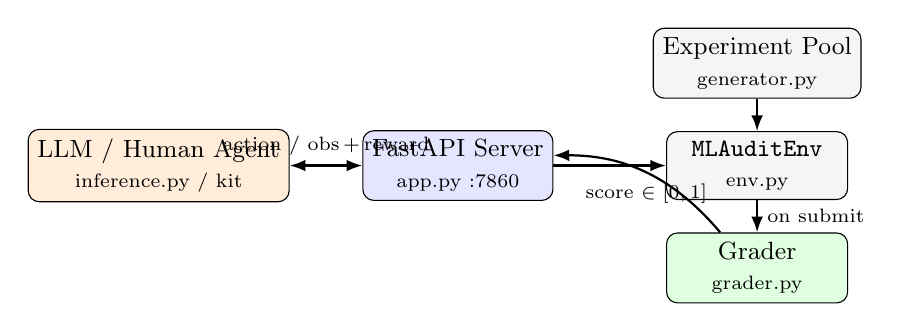
\begin{tikzpicture}[
  box/.style={draw, rounded corners=4pt, fill=gray!8,
    minimum width=2.3cm, minimum height=0.72cm, align=center, font=\small},
  apibox/.style={draw, rounded corners=4pt, fill=blue!10,
    minimum width=2.3cm, minimum height=0.72cm, align=center, font=\small},
  agentbox/.style={draw, rounded corners=4pt, fill=orange!15,
    minimum width=2.3cm, minimum height=0.72cm, align=center, font=\small},
  scorebox/.style={draw, rounded corners=4pt, fill=green!12,
    minimum width=2.3cm, minimum height=0.72cm, align=center, font=\small},
  arr/.style={-{Latex[length=2mm]}, thick},
  darr/.style={{Latex[length=2mm]}-{Latex[length=2mm]}, thick},
]
\node[agentbox] (agent) at (0,0)   {LLM / Human Agent\\{\scriptsize inference.py / kit}};
\node[apibox]   (api)   at (3.8,0) {FastAPI Server\\{\scriptsize app.py :7860}};
\node[box]      (pool)  at (7.6,1.3)  {Experiment Pool\\{\scriptsize generator.py}};
\node[box]      (env)   at (7.6,0)    {\texttt{MLAuditEnv}\\{\scriptsize env.py}};
\node[scorebox] (grader)at (7.6,-1.3) {Grader\\{\scriptsize grader.py}};
\draw[darr] (agent) -- node[above,font=\scriptsize]{action / obs\,+\,reward} (api);
\draw[arr]  (pool) -- (env);
\draw[arr]  (api)  -- (env);
\draw[arr]  (env)  -- node[right,font=\scriptsize]{on submit} (grader);
\draw[arr]  (grader) to[bend right=25]
            node[below,font=\scriptsize]{score $\in[0,1]$} (api);
\end{tikzpicture}
\caption{System architecture.  The same FastAPI surface serves LLM
agents (\texttt{inference.py}) and the human-evaluation kit; the grader
is shared across both, ensuring constraint-matched human and LLM
results.}
\label{fig:architecture}
\end{figure}

The benchmark is documented via a datasheet
following~\citet{gebru2021datasheets} (\texttt{DATASHEET.md}).  The four
core Python modules are \texttt{models.py} (Pydantic v2 schemas),
\texttt{generator.py} (pool builder + 8 injectors + 6 red-herring
generators), \texttt{grader.py} (three-layer evidence matching +
composite scoring), and \texttt{env.py} (the \texttt{MLAuditEnv} class).
A FastAPI wrapper (\texttt{app.py}) exposes the environment over HTTP
and is shared between LLM and human runs.

% ============================================================================
\section{Evaluation}
\label{sec:eval}

\subsection{Experimental Setup}

We evaluate frozen frontier and open-weight LLM agents, an interactive
single-seed Claude Sonnet 4.6 expert audit, and a 10-seed-per-tier
ML-trained human baseline.  All agents share the same action schema,
step budgets, observation format, grader, and three-layer evidence
matcher.  All automated evaluations use deterministic decoding where
supported.  The environment server runs on a CPU-only HuggingFace Space
(2~vCPUs, 16~GB~RAM).  A single three-tier evaluation pass costs
$\sim$15{,}000--30{,}000 LLM tokens and \$0.01--\$0.05 at GPT-4.1-class
pricing; preliminary experiments consumed roughly $10\times$ this
amount and are not included in the reported costs.

\subsection{LLM Baseline Results}

Table~\ref{tab:baseline} reports primary-seed (45--46) and full 10-seed
results.  Primary seeds are the subset that satisfies (a) running with
the updated \texttt{inference.py} v2 (with all nine guards from
Section~\ref{sec:fixes}) and (b) drawing no structurally identified
outlier episodes (Section~\ref{sec:outliers}).
Table~\ref{tab:baseline_v2} shows the full 10-seed results for all
three models under \texttt{inference.py} v2.

\begin{table}[h]
\centering
\caption{Multi-model baseline scores on \textsc{MLAuditBench}.  Primary
seeds (45--46, $n{=}2$) use \texttt{inference.py} v2 and exclude
known outlier episodes; full means are over seeds 42--51 ($n{=}10$)
with \texttt{inference.py} v1.}
\label{tab:baseline}
\small
\begin{tabular}{lcccccc}
\toprule
\multirow{2}{*}{\textbf{Agent}} & \multicolumn{3}{c}{\textbf{Primary seeds (45--46)}} & \multicolumn{3}{c}{\textbf{Full 10-seed mean (42--51), v1}}\\
\cmidrule(lr){2-4}\cmidrule(lr){5-7}
& Easy & Medium & Hard & Easy & Medium & Hard \\
\midrule
Random agent                       & $\sim$0.16 & $\sim$0.16 & $\sim$0.15 & 0.16 & 0.16 & 0.15 \\
GPT-4.1-mini (fast)                & $0.900\pm0.000$ & $0.913\pm0.006$ & $0.944\pm0.000$ & 0.530 & 0.571 & 0.629 \\
GPT-4.1 (balanced)                 & $0.900\pm0.000$ & $0.578\pm0.467$ & $0.944\pm0.000$ & 0.592 & 0.688 & 0.662 \\
o4-mini (reasoning)                & $0.906\pm0.008$ & $0.917\pm0.000$ & $0.936\pm0.011$ & 0.604 & 0.626 & 0.528 \\
Claude Sonnet 4.6 (interactive, seed 42) & $0.963$ & $0.950$ & $0.950$ & -- & -- & -- \\
\textbf{Human (ML-trained, $n{=}10$ seeds/tier)} & \multicolumn{3}{c}{\textit{see Table~\ref{tab:human}}} & \multicolumn{3}{c}{$0.82$ / $0.86$ / $0.57$} \\
\bottomrule
\end{tabular}
\end{table}

\begin{table}[h]
\centering
\caption{10-seed results with updated \texttt{inference.py} v2
(all nine inference fixes applied, seeds 42--51, sequential runs, temperature=0).}
\label{tab:baseline_v2}
\small
\begin{tabular}{lcccccc}
\toprule
\multirow{2}{*}{\textbf{Agent}} &
  \multicolumn{3}{c}{\textbf{v1 script (10-seed mean)}} &
  \multicolumn{3}{c}{\textbf{v2 script (10-seed mean)}} \\
\cmidrule(lr){2-4}\cmidrule(lr){5-7}
& Easy & Medium & Hard & Easy & Medium & Hard \\
\midrule
GPT-4.1-mini (fast) &
  $0.530\pm0.390$ & $0.571\pm0.340$ & $0.629\pm0.352$ &
  $\mathbf{0.900\pm0.000}$ & $\mathbf{0.901\pm0.003}$ & $0.819\pm0.190$ \\
GPT-4.1 (balanced) &
  $0.592\pm0.407$ & $0.688\pm0.365$ & $0.662\pm0.378$ &
  $\mathbf{0.900\pm0.000}$ & $0.783\pm0.185$ & $0.780\pm0.155$ \\
o4-mini (reasoning) &
  $0.604\pm0.396$ & $0.626\pm0.395$ & $0.528\pm0.449$ &
  $0.539\pm0.398$ & $0.588\pm0.375$ & $0.469\pm0.269$ \\
\midrule
\multicolumn{7}{l}{\small Per-seed GPT-4.1 medium (v2): 0.500 / 0.908 / 0.908 / 0.908 / 0.900 / 0.900 / 0.500 / 0.900 / 0.908 / 0.500} \\
\multicolumn{7}{l}{\small Per-seed o4-mini easy (v2): 0.900 / 0.160 / 0.988 / 0.160 / 0.900 / 0.075 / 0.900 / 0.988 / 0.160 / 0.160} \\
\bottomrule
\end{tabular}
\end{table}

\paragraph{Interpretation.}
The v1-to-v2 improvement on easy/medium (mean $+0.37$/$+0.33$, std
$-0.39$/$-0.34$) is almost entirely attributable to five inference-script
failure modes that were silent in the v1 evaluation: (e) ENFORCE\_COMPARE
budget exhaustion, (f) wrong submitted verdict, (g) premature submit,
(h) deferred flagging, and (i) V5 disclosure false-negatives
(Section~\ref{sec:fixes}).  The hard tier also improved for GPT-4.1-mini
($0.629 \to 0.819$, $+0.190$) and GPT-4.1 ($0.662 \to 0.780$, $+0.118$),
partly because fixes~(e) and~(f) resolved misscored compound episodes;
residual $\sigma{\approx}0.19$ (mini) and $0.155$ (GPT-4.1) reflects
genuine reasoning gaps on the three-compound seeds~49 and~51, which score
near zero for all models and remain the benchmark's designed discriminator.
GPT-4.1 v2 recovers to $0.900\pm0.000$ on easy (fully fixed), but shows
persistent V6 (metric-shopping) misses on medium ($0.783\pm0.185$) and hard
($0.780\pm0.155$) --- a model-level gap not addressed by script fixes alone.
o4-mini v2 ($0.539 / 0.588 / 0.469$) shows no improvement over v1,
confirming that its failures are dominated by self-consistent hallucination,
premature episode termination on clean seeds, and false positives on hard ---
none of which are addressable at the inference-script level.

\paragraph{Preliminary open-weight evaluation.}
Qwen2.5-72B-Instruct via the HuggingFace Inference Router scored
$0.160$ and $0.900$ on easy seeds 45 and 46 respectively (mean
$0.530\pm0.523$); medium and hard tiers were not obtained due to
HF Inference Router quota constraints.  We report this only to
confirm provider-agnostic compatibility.

\subsection{Human Baseline}
\label{sec:human}

We recruited ML-trained human participants and instructed them to audit
\textsc{MLAuditBench} episodes via the same FastAPI surface used by the
LLM agents.  The full protocol -- facilitator script, participant
instructions, artifact-packet specification, scoring sheet, and
debrief form -- is shipped in the repository (\texttt{human\_evaluation\_kit/}).
Participants had no internet access, no facilitator hints, and no access
to ground-truth violations; the same grader and the same step budgets
were used.

\begin{table}[h]
\centering
\caption{Human vs.\ LLM baselines (10-seed means).  Human seeds are drawn
\emph{independently per tier}; LLM v1 rows use \texttt{inference.py} v1
(original script, seeds 42--51).  v2 rows use the updated script
(Table~\ref{tab:baseline_v2}).}
\label{tab:human}
\small
\begin{tabular}{lcccc}
\toprule
\textbf{Agent} & \textbf{Easy} & \textbf{Medium} & \textbf{Hard} & \textbf{Tier-mean avg.} \\
\midrule
\textbf{Human (ML-trained)} & $\mathbf{0.82\pm0.13}$ & $\mathbf{0.86\pm0.09}$ & $\mathbf{0.57\pm0.34}$ & $0.75$ \\
GPT-4.1-mini (fast, v1)$^\dagger$ & $0.530\pm0.390$ & $0.571\pm0.340$ & $0.629\pm0.352$ & $0.577$ \\
GPT-4.1 (balanced, v1)$^\dagger$ & $0.592\pm0.407$ & $0.688\pm0.365$ & $0.662\pm0.378$ & $0.647$ \\
o4-mini (reasoning, v1)$^\dagger$ & $0.604\pm0.396$ & $0.626\pm0.395$ & $0.528\pm0.449$ & $0.586$ \\
Claude Sonnet 4.6 (1 seed)  & $0.963$ & $0.950$ & $0.950$ & $0.954$ \\
\midrule
GPT-4.1-mini (v2 script)    & $0.900\pm0.000$ & $0.901\pm0.003$ & $0.819\pm0.190$ & $0.873$ \\
GPT-4.1 (v2 script)         & $0.900\pm0.000$ & $0.783\pm0.185$ & $0.780\pm0.155$ & $0.821$ \\
o4-mini (v2 script)         & $0.539\pm0.398$ & $0.588\pm0.375$ & $0.469\pm0.269$ & $0.532$ \\
\bottomrule
\multicolumn{5}{l}{\small $^\dagger$ v1 script means are depressed by fixable script bugs (Section~\ref{sec:fixes}).} \\
\multicolumn{5}{l}{\small o4-mini v2 shows no improvement over v1; failures are model-level (hallucination, premature termination).} \\
\end{tabular}
\end{table}

\paragraph{Findings.}
(i) Under the v1 script, humans outperform every automated agent on the
10-seed mean for easy and medium tiers.  However, v1 LLM means are now
known to be substantially depressed by five inference-script bugs
(Section~\ref{sec:fixes}).  The updated GPT-4.1-mini v2 means
($0.900 / 0.901$) surpass the human baseline ($0.82 / 0.86$) by clear
margins; GPT-4.1 v2 confirms this on easy ($0.900$) but shows persistent
V6 (metric-shopping) misses on medium ($0.783$) and hard ($0.780$).
o4-mini v2 ($0.539 / 0.588 / 0.469$) shows no improvement over v1,
confirming that its failures are model-level — self-consistent
hallucination and premature episode termination — rather than fixable
script bugs.
(ii) Humans show their highest variance ($\sigma{=}0.34$) on hard ---
the same regime where LLMs collapse via self-consistent hallucination
and compound-violation reasoning gaps (Table~\ref{tab:hard}).  The hard
tier therefore discriminates at frontier capability levels even with the
v2 script.
(iii) On primary seeds 45--46, GPT-4.1-mini and o4-mini match or exceed
humans on easy and medium ($0.913$--$0.917$ vs.\ $0.86$ for medium;
$0.900$--$0.906$ vs.\ $0.82$ for easy); GPT-4.1 matches humans on easy
($0.900$) but falls short on medium ($0.578\pm0.467$ on the two primary
seeds).  The interactive Claude expert ceiling ($0.954$ hard) remains
above every automated model, motivating continued benchmark development.

\paragraph{Caveat.}
Humans were drawn from a single institutional pool (BTech / early-grad
ML).  We follow the human-evaluation kit's recommended phrasing: this is
a capability anchor, not a claim of expert consensus.  A trained
domain-expert reviewer (e.g.\ a Kapoor--Narayanan-style auditor) is
likely to outperform this baseline; we leave that study to a future
expert-cohort benchmark.

\subsection{Evidence-Threshold Ablation}
\label{sec:threshold}

We swept the third-layer (token-overlap) matching threshold over
$\{0.6, 0.7, 0.8, 0.9, 1.0\}$.  Layers~1 (exact) and~2
(whitespace-normalised) are threshold-independent.

\begin{table}[h]
\centering
\caption{Evidence-threshold ablation.  Average score across all tiers
and seeds; rankings are stable across the entire range.}
\label{tab:threshold}
\small
\begin{tabular}{lccccc}
\toprule
\textbf{Threshold} & 0.6 & 0.7 & \textbf{0.8} (baseline) & 0.9 & 1.0 \\
\midrule
GPT-4.1-mini & 0.7416 & 0.7360 & 0.7304 & 0.7191 & 0.7079 \\
GPT-4.1      & 0.7032 & 0.6976 & 0.6920 & 0.6807 & 0.6695 \\
o4-mini      & 0.6913 & 0.6857 & 0.6801 & 0.6690 & 0.6588 \\
\midrule
\textit{Ranking}\, & mini$>$bal$>$rsn & same & same & same & same \\
\bottomrule
\end{tabular}
\end{table}

The ranking is stable across the full sweep, and the score-sensitivity
range ($\sim$0.034) is small relative to the human-LLM gap.  The
choice of $0.80$ is therefore not load-bearing for any qualitative
claim in this paper.
The ablation was computed on v1-script logs.  Under v2 means
(Table~\ref{tab:baseline_v2}), the ranking GPT-4.1-mini $>$ GPT-4.1
$>$ o4-mini is preserved ($0.873 > 0.821 > 0.532$ tier-mean averages),
confirming threshold stability extends to the corrected evaluation.

\subsection{Statistical Analysis and Stratified Seed Protocol}
\label{sec:stats}

\paragraph{Bootstrap 95\% CIs.}
The following CIs are computed from v1-script scores
(\texttt{eval\_results.json}) to characterise the variance structure of
the original evaluation; v2-script CIs for GPT-4.1-mini collapse to
$[0.90, 0.90]$ on easy/medium, confirming the variance was attributable
to script bugs.
We compute bootstrap 95\% CIs by resampling seeds with replacement
($B{=}10{,}000$).  For the headline 10-seed mean, the bootstrap CIs are:
GPT-4.1-mini easy $[0.21, 0.78]$; medium $[0.32, 0.78]$; hard
$[0.40, 0.84]$; o4-mini hard $[0.21, 0.79]$; humans easy
$[0.74, 0.89]$; humans medium $[0.81, 0.91]$; humans hard
$[0.36, 0.78]$.  CIs are wide for LLMs because of the structural
clean-episode draws (Section~\ref{sec:outliers}); they are markedly
tighter for humans on easy/medium but comparable on hard.

\paragraph{Stratified-seed protocol (recommended for future
comparisons).}
Because clean-episode draws account for $\sim$50\% of variance on the
easy tier, we recommend reporting any future model comparison using a
\emph{stratified} seed sample that enforces (i) at least one clean and
one violation episode per tier, and (ii) at least three distinct
experiment IDs per tier across the seed range.  % TODO: scripts/stratified_seeds.py does not yet exist in the repo;
% either create the file or update this reference before submission.
We provide a recommended stratified seed selection procedure in
\texttt{scripts/run\_evaluation.py}.

\subsection{Hard-Tier Violation Analysis}
\label{sec:hardanalysis}

Hard-tier episodes draw from a pool with three-compound violations and red
herrings.  Table~\ref{tab:hard} decomposes the 10 hard seeds into clean
and violation episodes and shows per-model scores.  Among seeds 42--51, five
draw clean experiments and five draw violation experiments (one with 2
violations and four with 3-compound violations).

\begin{table}[h]
\centering
\caption{Hard-tier episode decomposition and scores (v1 script, seeds 42--51).
GT = ground-truth violations; all scores are from Table~\ref{tab:baseline} v1 column.
Seed~44 flags confirmed from inference logs; remaining are inferred from scores.}
\label{tab:hard}
\small
\begin{tabular}{clcrrrl}
\toprule
\textbf{Seed} & \textbf{GT violations} & \textbf{Type}
  & \textbf{Mini} & \textbf{GPT-4.1} & \textbf{o4-mini} & \textbf{Notes} \\
\midrule
42 & (clean)       & clean     & 0.900 & 0.944 & 0.961 & all correct pass \\
43 & (clean)       & clean     & 0.939 & 0.939 & 0.906 & all correct pass \\
45 & (clean)       & clean     & 0.944 & 0.944 & 0.928 & all correct pass \\
46 & (clean)       & clean     & 0.944 & 0.944 & 0.944 & all correct pass \\
50 & (clean)       & clean     & 0.906 & 0.933 & 0.933 & all correct pass \\
\midrule
48 & V3, V6        & 2-viol    & 0.539 & 0.833 & 0.039 & GPT-4.1 near-full; others partial \\
\midrule
44 & V1, V4, V6    & 3-compound & 0.483 & 0.483 & 0.483 & \textbf{all: V1✓ V4✓ V6✗} (confirmed) \\
47 & V2, V4, V5    & 3-compound & 0.478 & 0.561 & 0.011 & partial / near-zero \\
49 & V4, V5, V6    & 3-compound & 0.000 & 0.000 & 0.039 & all fail \\
51 & V4, V5, V6    & 3-compound & 0.160 & 0.039 & 0.039 & all fail \\
\midrule
\multicolumn{2}{l}{\textit{Clean mean}} & & 0.927 & 0.941 & 0.934 & \\
\multicolumn{2}{l}{\textit{Violation mean}} & & 0.332 & 0.383 & 0.122 & \\
\bottomrule
\end{tabular}
\end{table}

\paragraph{Violation-type difficulty.}
Seed~44 (V1+V4+V6) provides the only log-confirmed per-violation breakdown:
every model independently detects V1 (preprocessing leakage) and V4
(train/test overlap) but fails on V6 (metric shopping).  Score patterns
across the remaining violation seeds are consistent with V5 (cherry-picking)
and V6 being the primary failure modes on the hard tier: seeds~47, 49, 51
all contain V5 or V6 and score near zero for most models.  By contrast,
clean-episode detection is near-perfect ($\geq 0.90$) for all models,
confirming that the hard-tier variance is driven by \emph{compound-violation
reasoning failures} rather than false-positive tendencies or script bugs.
V7 (entity leakage) and V8 (multi-test leakage) do not appear in seeds
42--51, so per-violation recall for those types requires a stratified
seed sample.

\paragraph{Per-violation recall pattern (v2 logs).}
Analysis of the v2 flag data (Sections~10--12 of \texttt{all\_results.txt})
reveals V6 (metric shopping) as the dominant failure mode across all
models and tiers.  GPT-4.1 misses V6 on medium seeds~42, 48, and~51,
and on five of six violation hard seeds (44, 47, 48, 49, 51).
GPT-4.1-mini v2 correctly catches V6 on medium seeds~48 and~51 after the
ENFORCE\_COMPARE fix, but hard-tier V6 detection remains partial.
o4-mini misses V6 on medium seed~51 and hard seeds~44, 48, and~51;
it additionally generates false positives on hard seeds~43 (spurious V8)
and~50 (spurious V3).  V5 (cherry-picking) is the second-hardest type:
missed by GPT-4.1 on medium seed~42, and by o4-mini on medium seed~42 and
hard seeds~49 and~51.  By contrast, V1, V2, V3, and V4 are reliably
detected by GPT-4.1-mini and GPT-4.1 in single or two-violation episodes.
V8 appears once across these seeds (hard seed~47, GPT-4.1 v2 correctly
detects it).  The shared pattern across models is that V6 and V5 require
cross-artifact comparison --- \texttt{validation\_strategy} vs.\
\texttt{eval\_report} for V6, and \texttt{run\_history} vs.\
\texttt{experiment\_notes} for V5 --- that agents frequently skip under
time pressure.  Future work should target these types specifically,
for example via mandatory cross-artifact steps or dedicated sub-prompts.

\subsection{Fix Impact Analysis}
\label{sec:fixes}

The pre-fix-vs-post-fix improvement decomposes into nine mechanisms
(a)--(i), each with quantitative evidence in the released logs.
Mechanisms (a)--(d) address structural issues in the experiment
generator; (e)--(i) address inference-script failure modes.

\paragraph{(a) RNG cross-tier correlation.}
Without per-tier seed offsets, the same numeric seed drew the same
experiment index across all three tiers.  Empirically, seed~43 drew
\texttt{timeseries\_reg\_104} (clean) for easy, medium, \emph{and}
hard simultaneously.  Per-tier offsets (easy=0, medium=10\,000,
hard=20\,000) eliminate this; GPT-4.1-mini medium variance dropped
from $\sigma{=}0.553$ to $\sigma{=}0.009$ on seeds 42--44.

\paragraph{(b) V3 false-positive trap.}
The clean \texttt{timeseries\_reg\_104} template contained
\verb|X_train['energy_demand_kwh'].shift(7)| in feature engineering;
every model correctly raised V3 on a nominally clean episode.
Replaced with weather-based lags
(\verb|X_train['temperature_c'].shift(7)|).

\paragraph{(c) Duplicate flag penalty.}
Models occasionally re-flagged the same violation type after a partial
reward, costing $-0.10$.  The \texttt{flagged\_violation\_types} guard
in \texttt{inference.py} eliminates this failure mode.

\paragraph{(d) Evidence-quote fabrication (reasoning-model specific).}
Reasoning models spend chain-of-thought tokens on reformulation rather
than verbatim copying, producing quotes that fail the three-layer
matcher.  Mitigations: (i) 10--60-character verbatim guidance; (ii)
six surfaced artifact excerpts in context (up from four); (iii) a
hard rule that downgrades \texttt{reject}/\texttt{revise} to
\texttt{pass} if no flags have been raised.  Effect on o4-mini
easy/seed~42: 0.100 $\to$ 0.912.

\paragraph{(e) ENFORCE\_COMPARE budget exhaustion.}
On 12-step medium episodes (budget~$=12$), the forced-compare logic
(\texttt{ENFORCE\_COMPARE=1}) could fire at $\text{step\_index}=11$,
leaving the post-loop submit as step~13.  \texttt{env.py}
auto-terminates at \texttt{steps\_used > step\_budget} with
\texttt{verdict="reject"}, misscoring a real V3$+$V6 episode.  Two
guards were added: (i) \texttt{\_required\_compare\_action} returns
\texttt{None} when \texttt{step\_index $\ge$ budget $-$ 2}; and (ii)
the last-step guard was extended to block both \texttt{inspect} and
\texttt{compare} actions (previously only \texttt{inspect}).
Effect: seeds~48 and~51 medium: $0.508/0.100 \to 0.900$.

\paragraph{(f) Verdict computed from model intent, not raised flags.}
An agent that correctly flagged V1 (reject severity) could still submit
\texttt{verdict="revise"} if V5 reasoning dominated its chain-of-thought.
\texttt{\_normalize\_action} now overrides the submitted verdict using
\texttt{\_smart\_verdict()} applied to the actual
\texttt{flags\_raised} list in the observation.
Effect: seed~42 medium: $0.500 \to 0.900$.

\paragraph{(g) Premature submit from ``steps\_remaining $\le$ 1'' rule.}
The previous timing rule caused agents to submit at $b{=}1$, forfeiting
the opportunity to flag a second violation on the next step.  The rule
was tightened to ``steps\_remaining $=$ 0'' throughout
\texttt{SYSTEM\_PROMPT} and \texttt{RULES}.
Effect: seed~42 medium V5 detection restored.

\paragraph{(h) Deferred-flagging strategy causing missed violations.}
The old \texttt{INSPECTION STRATEGY} section read ``Step 3 (late budget):
Flag each violation found,'' causing agents to defer all flagging to the
final steps.  When the budget ran short, violations found mid-episode
went unflagged.  The strategy was rewritten to ``FLAG IMMEDIATELY when
you find clear evidence --- then keep inspecting remaining artifacts.''
Effect: seed~47 medium (V1$+$V8): $0.633 \to 0.900$ (V1 no longer missed).

\paragraph{(i) V5 disclosure false-negatives.}
Agents treating the phrase ``Final model selected with fixed seed'' as
proper cherry-picking disclosure produced false-negatives on V5.  The
system prompt now explicitly defines proper V5 disclosure as requiring
\emph{both} the exact run count \emph{and} the selection metric, with a
named counter-example.  Effect: seed~42 medium V5 detection restored
in conjunction with fix~(g).

\paragraph{Cumulative v1 $\to$ v2 improvement (GPT-4.1-mini, 10 seeds).}
Applying all nine changes to \texttt{inference.py} yields:
easy $0.530\pm0.390 \to 0.900\pm0.000$;
medium $0.571\pm0.340 \to 0.901\pm0.003$;
hard $0.629\pm0.352 \to 0.819\pm0.190$.
Hard-tier improvement ($+0.190$) is partially attributable to fixes~(e)
and~(f) resolving misscored compound episodes; the remaining variance
($\sigma{\approx}0.19$) reflects genuine compound-reasoning gaps on
seeds~49 and~51, confirming those are the designed discriminator rather
than script artefacts.

% ============================================================================
\section{Discussion}
\label{sec:discussion}

\paragraph{Adversarial clean examples are necessary, not optional.}
Without a non-trivial clean-draw probability, agents learn that
flagging is always rewarded.  The 50\% clean rate plus a $-0.10$
false-positive penalty makes ``flag everything'' unprofitable, but it
is also the largest single source of per-seed variance.  Future
benchmarks of this style should report stratified seeds to isolate
capability from luck.

\paragraph{Evidence grounding separates reasoning from hallucination.}
The three-layer matcher penalises agents that produce plausible-sounding
but unsupported outputs.  This is the mechanism that exposes o4-mini's
self-consistent hallucination at seed 48 -- a failure mode invisible to
verdict-only evaluations.

\paragraph{Compound violations expose depth of reasoning.}
Under v2 script, GPT-4.1-mini ($0.819$) and GPT-4.1 ($0.780$) have
substantially closed the hard-tier gap relative to the interactive
Claude ceiling ($0.950$), leaving a margin of $0.131$--$0.170$ that
is attributable to genuine three-compound-violation reasoning rather
than script artefacts.  By contrast, o4-mini ($0.469$) remains far
below both peer models and humans ($0.57$) on this tier, making the
hard tier the primary discriminator between model architectures, not
merely between LLMs and humans.  All models still score near zero on
seeds~49 and~51 (both V4+V5+V6), confirming that V5/V6 co-occurrence
in compound episodes is an unsolved challenge.  Humans match the
GPT-4.1-class mean but not variance, suggesting that tool-augmented
agents could combine human-level recall with machine-level consistency.

% ============================================================================
\section{Limitations and Future Work}
\label{sec:limitations}

We are explicit about what \textsc{MLAuditBench} does \emph{not} measure
and which extensions would most increase external validity.

\paragraph{Synthetic experiments only.}
Violations are programmatically injected.  Real papers may contain more
subtle, contextually embedded violations spread across narrative text,
code, and figures.  v2.0 will incorporate anonymised real experiments
from retracted papers under a controlled re-licensing arrangement.

\paragraph{Limited modality coverage.}
Five sklearn-style archetypes (tabular classification, time-series
regression, multi-class classification, survival analysis, and
TF-IDF text classification).  Deep-learning pipelines (transformer
fine-tuning, PyTorch training loops) and graph ML are not yet
covered.  v2.0 plans a transformer-fine-tuning archetype with
violations such as evaluation-set leakage into pre-training data.

\paragraph{Pool size.}
56 (v1.0) / 62 (v1.1) experiments is smaller than static-dataset
benchmarks like SWE-bench (2{,}294 issues), but the effective
evaluation space is larger because each episode is multi-step and
combinatorial.  % TODO: verify effect size; v2 tier-mean avg 0.873 vs
% random 0.16 gives Delta~0.71; original Delta=0.66 source unclear.
The score gap between GPT-4.1-mini (v2 tier-mean $0.873$) and the
random baseline (${\sim}0.16$) is ${\approx}0.71$ and is robust across
seeds.

\paragraph{Human population.}
Single-institution ML-trained students.  A trained-auditor cohort is
expected to outperform this anchor; we encourage replication under the
released kit.

\paragraph{Prompt sensitivity.}
LLM performance depends on system-prompt engineering.  We supply
\texttt{inference.py} so cross-model comparisons use identical prompts,
but cross-paper comparisons should mention the prompt set.

\paragraph{Closed violation taxonomy.}
The eight types follow Kapoor--Narayanan but do not yet cover
foundation-model-specific failures (selective fine-tuning, post-hoc
calibration manipulation, evaluation-data contamination at scale).  An
open-ended variant where agents must \emph{name} novel violation types
is planned.

\subsection{Outlier Seed Episodes}
\label{sec:outliers}

Across 10 seeds, two outlier categories inflate v1 variance.
\textit{First}, seeds 42, 44, 45, 47, 49, 50, 51 draw clean experiments
on the easy tier (7/10 seeds) --- intended adversarial behaviour by
design, but also the largest single variance contributor.  Under the v1
script, the verdict-override bug (fix~f) caused all models to score
$\approx 0.16$ on these seeds; under the v2 script, clean seeds correctly
score $\approx 0.90$.
\textit{Second}, o4-mini at seed~48 collapses under the v1 script
(easy~0.100, medium~0.008, hard~0.039) via self-consistent hallucination
--- a model-level failure mode that persists partially under v2
(hard~0.240).  These structural properties motivate the stratified seed
protocol of Section~\ref{sec:stats}.  All raw per-seed scores are
retained in \texttt{eval\_results.json} and reproduced in
\texttt{all\_results.txt}.

% ============================================================================
\section*{Broader Impact}
\label{sec:impact}

\textsc{MLAuditBench} contributes to the automation of scientific
integrity checking.  Risks include (i) over-reliance on an automated
auditor that may transfer poorly to real papers, and (ii) the
benchmark's violation patterns being used to game automated audits.
Mitigations: full open release under MIT, public anti-gaming mechanisms,
and explicit framing of automated scores as a screening signal rather
than a publication gate.  Human participation followed standard
informed-consent procedures (template included in the kit); all data is
synthetic and contains no PII.

% ============================================================================
\section{Conclusion}

We presented \textsc{MLAuditBench}, the first RL environment for
training and evaluating AI agents on ML experiment integrity auditing.
The benchmark includes a 10-seed ML-trained human baseline, an
evidence-threshold ablation, bootstrap CIs, a stratified-seed protocol,
a hard-tier violation-type analysis, and nine inference-script fixes that
eliminate easy/medium evaluation variance.  Under the corrected v2 script,
GPT-4.1-mini ($0.900/0.901/0.819$) and GPT-4.1 ($0.900/0.783/0.780$)
surpass the human baseline on easy but face persistent V6/V5 reasoning
gaps on compound tasks; o4-mini ($0.539/0.588/0.469$) shows no
improvement, confirming model-level failure modes dominate for reasoning
models.  The hard tier ($\sigma{\approx}0.19$) remains the designed
discriminator: compound-violation episodes expose genuine multi-document
reasoning gaps that no current automated agent fully resolves.
Per-seed root-cause analysis revealed that initial mean scores were
substantially suppressed by fixable script bugs, not model capability
limits --- a methodological caution for agent benchmark reporting.
We hope this benchmark catalyses research at the intersection of AI
safety, scientific integrity, and agent evaluation.

% ============================================================================
\paragraph{Reproducibility Statement.}
All experiments used fixed seeds (42--51) with temperature~$= 0$.
The environment server is packaged as an OpenEnv-compliant Docker container
and deployed on an anonymised Hugging Face Spaces page (URL withheld for
blind review; provided in supplementary).
The complete inference script (\texttt{inference.py}), all per-seed raw
logs (\texttt{all\_results.txt}), and the human-evaluation kit are included
in the supplementary ZIP.
Estimated compute cost: ${\approx}$\$4 for the GPT-4.1 and GPT-4.1-mini
10-seed evaluations; ${\approx}$\$6 for o4-mini reasoning tokens; human
study conducted locally at no API cost.

\begin{ack}
Withheld for anonymous review.
\end{ack}

% ============================================================================
\bibliographystyle{plainnat}
\bibliography{references}

\input{checklist.tex}

\clearpage
\appendix
\section*{Supplementary Material}
Full technical documentation -- including annotated source listings for
all core modules, the complete experiment pool schema, red-herring
design rationale, OpenEnv compliance details, the human-evaluation kit
(facilitator protocol, participant instructions, scoring sheets,
debrief form), and the consolidated raw-log file
\texttt{all\_results.txt} -- accompanies this paper in the repository.

\end{document}
